\section{\textbf{What} is quantum computing?}

\begin{fullwidth}

\textit{Quantum computing} sounds pretty intimidating to most people. What if I remove the ``quantum'' part, leaving only the ``computing'' part? 
Much friendlier, huh? 
The ``computing'' part is plain as simple: Give a system some input, and it will give you some output. 
Now comes the jargon, ``quantum''. The word ``quantum'' comes from \textit{Quantum Mechanics}, a branch of physics that study tiny things. 
Therefore, \textit{quantum computing} is essentially a way of using tiny particles to do calculation for us.
The quantum computer manipulates on subatomic particles to do calculations, so you can imagine it is EXTREMELY difficult to build a quantum computer.
Although there are prototypes of quantum computer as year of 2018, none of them has real application yet.
However, quantum computing is not that far away from us.
In fact, people believe it will become an critical technology in the following decades.

\end{fullwidth}

\section{\textbf{Why} quantum computing?}

\begin{marginfigure}[15\baselineskip]
    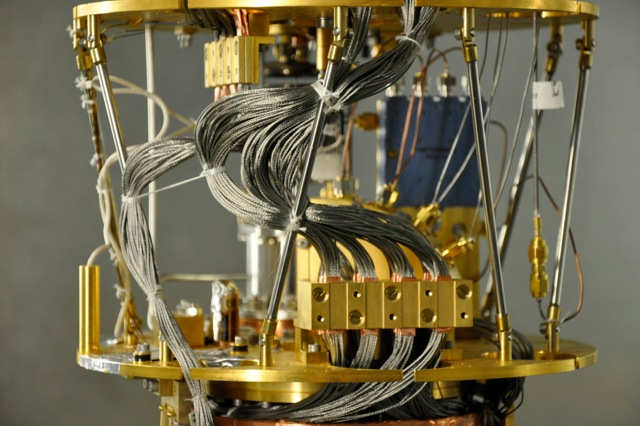
\includegraphics[width=\linewidth]{chapter1/quantum-computer-picture}
    \caption{Support structure for a D-WAVE quantum computer.}
    \label{fig:chapter1-quantum-computer-picture}
\end{marginfigure}

In short, quantum computer (Figure \ref{fig:chapter1-quantum-computer-picture}\cite{Chapter1-quantum-computer-picture}) can solve problems we can never solve with classical computer.
For example, there is an encryption algorithm we use everywhere, everyday, called RSA algorithm.
By using RSA algorithm, our passwords are encrypted during transmission and keep our money/data safe.
It is safe because it will take centuries for the most powerful super computer to decrypt the message encrypted by RSA.
But for quantum computer? This decryption process could be just a matter of seconds. 
What does that mean? If you have a quantum computer today, you would be able to hack almost all bank accounts on earth.
Of course, we don't want to build a quantum computer only good for hacking bank accounts, right?
There are a number of other applications like climate simulation, machine learning, material research, etc.
You already know how computers change the world.
Then just imagine the world will be changed again by quantum computers, and embrace the future!

\section{\textbf{How} can we try quantum computing?}

\begin{fullwidth}

As of April 2018, there are a few options for us to write quantum programs on a simulated quantum computer.
Why simulated quantum computer? Because the real quantum computer doesn't exist yet!
Furthermore, using simulated quantum computer can get our hands dirty already.
The Q\# language from Microsoft will be used as the main language for quantum programs throughout the book.

\end{fullwidth}

\section{Introduction to quantum mechanics}

\begin{fullwidth}

Before playing around with quantum computing, we need to have some basic background in quantum mechanics.
But don't worry, let's go through the basics together.
Since the mathematical foundation of quantum mechanics is linear algebra, we are gonna learn linear algebra first.
Then we will use the powerful mathematical tool to explain a few important ideas in quantum mechanics.
Finally, we will apply our newly learned knowledge to write our first quantum program!
How cool is that!
So please bear with me for the theoretical part.
Otherwise, you will not understand how we code the quantum program.

\end{fullwidth}

\subsection{Linear algebra for quantum computing}
It could easily take a few months for normal people to learn linear algebra.
Therefore, we will only cover essential parts here.
There are numerous resources on linear algebra out there, if you want to learn more about it.
For example, the MIT open course: \href{https://ocw.mit.edu/courses/mathematics/18-06-linear-algebra-spring-2010/}{Linear Algebra 18.06} from Prof. Strang\cite{Chapter1-mit-linear-algebra} is extremely good, and you can benefit a lot by completing it.

\subsubsection{\textbf{What} is linear algebra?}

\section{Your first quantum program with Q\#}

\begin{fullwidth}

Now let's get down to business. It's time to write our first quantum program!
But first things first, let me give you an overview of Q\#.
Q\# is a quantum programming language.
This means that Q\# is designed to express quantum algorithm or logic instead of classical computation.
The Q\# language is NOT a program language that we can use for implementing classical algorithms.
Therefore, when we want to write a complete quantum program, we might end up using some classical programming language along with quanutm programming language like Q\#.
For example, let's say you live in the U.S., and you want to visit China.
What you will probably do is to take a car ride to the airport, then take the plain to China, right?
In the example, the car is the classical language and the plain is the quantum language.
They both have their own strength, and only by working together they can get you to your destination.

\end{fullwidth}


Now let's do the coding.
This program is taken from Microsoft blog\cite{Chapter1-first-quantum-program}, but that blog assumes the reader has some quantum computing background.
So instead of redirecting you to the article, let's walk through the program together with our beloved rubber duck methodology\cite{Chapter1-rubber-duck}.

\begin{marginfigure}[\baselineskip]
    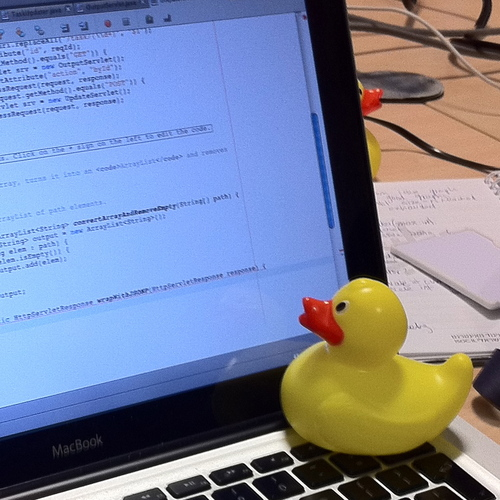
\includegraphics[width=\linewidth]{chapter1/rubber-duck-debugging}
    \caption{Rubber duck debugging}
    \label{fig:chapter1-rubber-duck-picture}
\end{marginfigure}

For those who doesn't know what rubber duck methodology is, I encourage you to spend a minute and search for rubber duck debugging\cite{Chapter1-rubber-duck-picture}.

\subsection{Setting up environment}
To setup a Q\# development environment, you need to install
\begin{enumerate}
  \item .NET core 2.0 SDK or later
  \item Visual Studio Code (For Windows users, you can use Visual Studio)
  \item Microsoft Quantum Development Kit Extension for Visual Studio Code/Visual Studio
\end{enumerate}
For detailed instructions, please refer to
\href{https://docs.microsoft.com/en-us/quantum/quantum-installconfig?view=qsharp-preview&tabs=tabid-vscode}{Installing and Validating the Q\# Development Environment}\cite{Chapter1-setup-environment}.

\subsection{Creating a Bell state}
